\documentclass[10pt,a4paper,twoside]{report}
\usepackage[utf8]{inputenc}

\usepackage[]{feupteses}
%\usepackage[square,sort,comma,numbers]{natbib}

\usepackage[english]{babel}
%\usepackage[T1]{fontenc}
\usepackage{amsmath}
\usepackage{amsfonts}
\usepackage{amssymb}
\usepackage{acronym}
\usepackage{graphicx}
\usepackage{float}
\usepackage{a4wide}
\usepackage{fancyhdr}
\usepackage[titles]{tocloft}
\usepackage{lastpage}
\usepackage{verbatim}
\usepackage[nodayofweek]{datetime}
\usepackage[bookmarks=true,colorlinks=true]{hyperref}
\numberwithin{figure}{chapter}
\usepackage{cite}

\usepackage{notoccite}

\usepackage{multirow}

%\usepackage{palatino}

\setcounter{tocdepth}{5} %shows all levels incl. paragraph

\usepackage{graphicx}
\usepackage{caption}
\usepackage{subcaption}
\usepackage{epstopdf}
\usepackage{xcolor}
%TESTE
\usepackage{scrextend}
\usepackage[absolute,overlay,showboxes]{textpos}

\setlength{\TPHorizModule}{10mm}
\setlength{\TPVertModule}{30cm}
\setlength{\parindent}{1mm}


%Aparecer até subsubsection no indice
\setcounter{secnumdepth}{3}
\setcounter{tocdepth}{2}
\usepackage{amsmath}
\usepackage{mathtools}

\newcommand{\HRule}[1]{\hfill \rule{0.1\linewidth}{#1}} % Horizontal rule at the bottom of the page, adjust width here

\usepackage{xcolor}
\definecolor{FEUP}{RGB}{140,45,25}

\hypersetup{citecolor=black}

\hypersetup{linkcolor=black,urlcolor=black}

\usepackage{graphics}

\usepackage{titlesec}
\titleformat{\chapter}[display]
  {\normalfont\Large\raggedleft}
  {\MakeUppercase{\chaptertitlename}%
    \rlap{ \resizebox{!}{1.5cm}{\thechapter} \rule{5cm}{1.5cm}}}
  {10pt}{\Huge}
\titlespacing*{\chapter}{0pt}{30pt}{20pt}
\usepackage{lipsum}
\setcounter{chapter}{0}


\setlength\parindent{24pt}


%%%%%%%%%%%%%%%%%%%%%%%%%%%%
\usepackage{graphicx}
\usepackage{framed}
\usepackage{multirow}
\usepackage{lipsum}  
\usepackage{verbatim}
\usepackage{amsmath}
\usepackage{longtable}
\usepackage{caption}
\usepackage{subcaption}
\usepackage{varwidth}

\usepackage{array}
\usepackage{adjustbox}

\usepackage{booktabs}
\usepackage{multirow}

\usepackage{mdframed}


\newcolumntype{L}[1]{>{\raggedright\let\newline\\\arraybackslash\hspace{0pt}}m{#1}}
\newcolumntype{C}[1]{>{\centering\let\newline\\\arraybackslash\hspace{0pt}}m{#1}}
\newcolumntype{R}[1]{>{\raggedleft\let\newline\\\arraybackslash\hspace{0pt}}m{#1}}






\include{report.macros}

\begin{document}

\pagenumbering{roman}
\thispagestyle{empty}

%----------------------------------------------------------------------------------------
%	TITLE SECTION
%----------------------------------------------------------------------------------------
\pdfbookmark[0]{Title}{Title}

\begin{textblock}{2}(0,0)%%%Places a vertical line
	\rule{0mm}{30cm}
	\textblockcolour{FEUP}
\end{textblock}

%FEUP FIGURE

{\color{white} - }
\vfill

\begin{figure}[ht!]
	\begin{addmargin}[2cm]{1mm}
		\begin{center}
			\includegraphics[scale=0.45]{figures/0.Title/FEUP.eps}
		\end{center}
	\end{addmargin}
	
\end{figure}

%TITLE OF THE DOCUMENT - Optimizing Energy Efficiency for Train Operation Constrained to Scheduling
\vspace{25mm}
\begin{addmargin}[2cm]{1mm}
	\begin{center}
		
		\begin{LARGE}
			\textbf{\color{FEUP} Railway Smart Meters\\}
		\end{LARGE}
		
		\vspace{5mm}
		
		\textbf{Thesis Work Plan\\}
		
		\vspace{30mm}
		
		\textbf{\Large Vítor A. Morais} \\
		
		\vspace{5mm}
		
		\textbf{Supervisor:} \textbf{Prof. António P. Martins (FEUP)} \\
		\textbf{Co-Supervisor:} \textbf{Prof. João L. Afonso (UMinho)}
		
		\vfill % Space between the title box and author information
		
		\small{Doctoral Program in Electrical and Computer Engineering,}\\
		\small{Department of Electrical and Computer Engineering}\\
		\small{Faculty of Engineering, University of Porto\\}
		\small{\today \par} %$31^{th}$ July, 2016
		
	\end{center}
	
\end{addmargin}

%----------------------------------------------------------------------------------------

\clearpage % Whitespace to the end of the page

%\input{Sections/abstract}
\cleardoublepage
\pdfbookmark[0]{Contents}{contents}
\tableofcontents
\cleardoublepage
\pdfbookmark[0]{List of Figures}{figures}
\listoffigures
\cleardoublepage
\pdfbookmark[0]{List of Tables}{tables}
\listoftables





%\chapter*{Abstract}
%Abstract goes here
%%
%%   Section 
%%
\begin{Prolog}
\cleardoublepage

\tableofcontents


%\printnomenclature

%\chapter*{Symbols}
%\begin{flushleft}

\begin{tabular}{l p{0.8\linewidth}}


kbps     & Kilobit per second (often used kbit/s or kb/s) - bit rate\\
Mbps     & Megabit per second (often used Mbit/s or Mb/s) - bit rate\\
Gbps     & Gigabit per second (often used Gbit/s or Gb/s) - bit rate\\
dB       & Decibel - Gain/Attenuation\\
kHz      & Kilohertz - Frequency\\
MHz      & Megahertz - Frequency\\
GHz      & Gigahertz - Frequency\\
km       & Kilometer - Distance\\
min      & Minute - Time\\


\end{tabular}
\end{flushleft}

	
\end{Prolog}

\StartBody

\chapter{Introduction}
\lipsum[4-4]


\chapter{Objectives and Contributions}





\section{Objectives}

This work is focused on measuring the energy flows in the railway system.
The aim of this work is to improve the energy efficiency in the railway transportation system (RTS) and reduce the maintenance cost of RTS power systems.
The implementation of smart meters (SM) in RTS promote a better overview of power flow and, based on the information of SM, algorithms focusing on energy efficiency can be implemented.
The SM requires sensors such as voltage and current sensors. The level of intrusion as well as the level of electric <<valor da grandeza electrica>> of such sensors implies considerable costs of the sensors.
Therefore, the implementation of complex processing on smart meters is of added value. This complex processing can be the implementation of fault monitoring algorithms in SM based on the energy measurements.
Framed in the shif2rail, the work is focused on the implementation of a smart meter demonstrator for the RTS. To embrace the entire railway system, the power flow should consider the energy flux from and to the catenary. Therefore, the key point should be the measurement of the energy in the traction substations and in the train power transformer 
Based on this thesis proposal, the objectives are the following:

\begin{itemize}
	\setlength\itemsep{0em}
	
	\item	Modeling, development and implementation of a metering system based on a non-intrusive self-powered sensor node.

	\item Modeling and simulation of a RTS wireless network.

	
\end{itemize}


\section{Contributions}

\begin{itemize}
	\setlength\itemsep{0em}
	
	\item Availability of measured data from trains where currently no energy measurement is performed.
	
	\item Data-rate increase of energy measurements, which will result on direct increase on the quality of information of energy.
	
	\item A further contribution can be the avoidance of broadband real-time/continuous communication (such as LTE), being possible to collect and store data in train data concentrator and, while the train is waiting at stations, the data is transferred between train and station AP (and then to a remote server). A possible contribution will be the cost reduction of information transmission of energy sensor network data.
	
	\item New advanced sensor node for AC current measurement;
	
	\item Possible contribution: Given the measurement characteristics, a self powered wireless sensor node can implement features of high processing.
	
\end{itemize}







\chapter{Literature Review}
\lipsum[4-4]





%\section{Synthesis}

%\lipsum[4-4]

















\section{Section 1: Smart metering}

In this section, special attention is given to smart metering. The smart grid framework is presented to justify the need for smart meters and then, an overview on metering systems is presented.


1.	Smart grids and the need for smart meters

2.	Metering systems – overview

3.	Metering systems in railways

4.	Wireless sensor networks – overview

5.	Smart metering with WSN in Railway Transportation System (RTS)

\subsection{Smart grids and the need for smart meters}

Smart Grids improves the functionality and concept of traditional electrical grids by obtaining the grid component's data using Information and Communication Technology (ICT). Such grids benefit the reliability and the efficiency of the system with the usage of the acquired data, \cite{Mohassel2014}.

Although the smart meters does not have an effective definition, those devices are composed by an electronic box and a communication link, \cite{Seppo2012}. A smart meter is responsible for measuring the energy-related parameters and the user consumption with a given time interval. All those measurements are then transmitted upon a communication network to the utility or to other player with the responsibility of using the meter data. The information obtained from the data is shared with consumer-side devices, to inform the end-users on their related costs and energy usage, \cite{Siano2014}.

Smart meters implement a bidirectional communication on top of AMR. They are inherent to smart grid systems. 

Similarly to the evolution of electricity meters, the utility grid has evolved from a centralized production and control perspective to a distributed one. The conventional electrical grid is a network with a transmission link connecting power producers and end-user consumers. The control and distribution of electrical power is made in a centralized way. With the increase of power demand, increase of complexity and having more and more decentralized power generation, a migration to the smart grid framework is required, \cite{Reddy2014}.

\subsection{Features of Smart Meters and metering systems}

A smart metering system combines several controlling devices, a extensive number of sensors for measuring the parameters and devices responsible for the transferring of the data and the commands. The detection of unauthorized consumption due to electrical energy theft and the improvement of the energy in the distribution are other advantages of smart meters. These devices acts as a gateway by having a communication interface protocol to the database stored by the utility company, \cite{Reddy2014}.

The design of an ideal smart grid has to focus on prediction, adaptability and reliability points. Moreover, it requires to cover the demand adjustment, the load handling, flexibility and sustainability and it should incorporate advanced services. In advance, an end to end control capability has to be ensured as well as finding the optimal cost and asses, increase the quality of energy and quality of service. Another features of smart grids are the automatic restoration ans self-healing, being all the previously presented features of the smart grids highly dependent of the role of the smart meters, \cite{Mohassel2014}.

Smart-meter types are also distinguished based on features like data-storage, communication type and connection with the energy supplier. The data storage capability allows data to be stored in the meter, being transferred after a few days or weeks to the Meter Data Management System (MDMS) of the utility. Compensations for some power quality deficiencies can be also considered; therefore the future meters should be also capable of register certain basic power quality characteristics. In advance, the design of rate and tariffs of electricity providers determine the requirements such as the period of meter intervals or the temporal resolution (commonly ranging from 15 min to 1 h). During those intervals, the production and consumption of active and reactive power is mandatory to be separately measured, \cite{Siano2014}.

\subsection{Metering systems in railways}


\subsection{Wireless sensor networks – overview}


\subsection{Smart metering with WSN in Railway Transportation System (RTS)}


%%%%%%%%%%%%%%%%%%%%%%%%%%%%%%%%
%%%%%%%%%%%%%%%%%%%%%%%%%%%%%%%%%
%%%%%%%%%%%%%%%%%%%%%%%%%%%%%%%%%





\section{Section 2: Wireless networks}

In this section, communication networks are presented, with special attention to wireless technologies. An historic overview is presented 



1.	Network technologies – historic overview

2.	Current technologies and standards:

3.	Emerging technologies and standards

4.	Network Simulators and Network Emulators






\subsection{Network technologies – historic overview}


\subsection{Current Wireless technologies and standards}

The following sections will cover the wireless communications in smart metering systems, starting with the low-rate and low-power communications applied around the smart meters and ending with the high-rate communications (and consequently higher costs and power than low rate communications). With the increasing on demand for higher bandwidth, broadband technologies such as mobile WiMAX, IEEE 802.16e and broadband PLC are expected to be considered and used in newer installations, \cite{Mohassel2014}.


%As the demand for bandwidth increases, broadband technologies such as IEEE 802.16e, mobile WiMAX and broadband PLC are going to play a key role in newer installations, \cite{Mohassel2014}.

\subsubsection{IEEE 802.11 (Wireless LAN (WLAN) or Wi-Fi)}

IEEE 802.11 is the standard for the information exchange between systems and for the telecommunications. The coverage area of this technology is on local and metropolitan area networks (LANs and MANs). The specific requirements are on the Medium Access Control and on Physical Layer. The most popular versions of this standard is the IEEE 802.11b and IEEE 802.11g, that differs in the modulation technique (Direct Sequence Spread Spectrum (DSSS) technique versus Orthogonal Frequency Division Multiplexing (OFDM) modulation technique). The data rates are, respectively, 11 Mbps and 54 Mbps, \cite{Usman2013, ieee2012}.



\subsubsection{IEEE 802.15.4 (ZigBee)}

The standard IEEE 802.15.4 imposes conditions in the physical layer and media access control focusing on low-rate (up to 300 kHz) wireless personal area networks. Developed by the Zigbee Alliance and covering the specifications of the IEEE 802.15.4 on the physical layer and the medium access control, Zigbee is a commonly used for low power wireless communication technology. It operates on the ISM bands of 868 MHz, 915 MHz and 2.4 GHz adopting direct sequence spread spectrum (DSSS), \cite{Usman2013}.

%IEEE 802.15.4 is a standard that specifies the physical layer and media access control for low-rate (up to 300kHz) wireless personal area networks. ZigBee is a popular, low power wireless communication technology developed by the ZigBee Alliance based on the Physical Layer and Media Access Control Layer of the IEEE 802.15.4 standard.
%It operates on the ISM bands of 868 MHz, 915 MHz and 2.4 GHz adopting direct sequence spread spectrum (DSSS), \cite{Usman2013}.


\subsubsection{DASH7}

On the low-rate field of research, an alternative to Zigbee is the DASH7. Using the ISO/IEC 18000-7 standard to support this wireless sensor network technology, DASH7 is developed to reach active Radio Frequency Identification Devices (RFIDs) and operates at 433MHz band. The advantage is the typical range of 250m (could achieve 5 km) and has a typical and maximum data rates of 28 kbps and 200 kbps, being in this specifically designed for Smart Grid and for applications in Smart Energy.


\subsubsection{6LoWPAN}

IEEE 802.15.3: IEEE 802.15.3 [46] is a physical and MAC
layer standard for high data rate WPAN. It is designed to
support real-time multi-media streaming of video and music.
IEEE 802.15.3 operates on a 2.4 GHz radio and has data
rates starting from 11 Mbps to 55 Mbps

\subsubsection{Wibree}

Wibree [47] is a wireless communication technology
designed for low power consumption, short-range
communication, and low cost devices. Wibree allows the
communication between small battery-powered devices
and Bluetooth devices. Small battery powered devices include
watches, wireless keyboard, and sports sensors
which connect to host devices such as personal computer
or cellular phones. Wibree operates on 2.4 GHz and has a
data rate of 1 Mbps. The linking distance between the devices
is 5–10 m. Wibree is designed to work with Bluetooth.
Bluetooth with Wibree makes the devices smaller
and more energy-efficient. Bluetooth–Wibree utilizes the existing Bluetooth RF and enables ultra-low power consumption.
Wibree was released publicly in October 2006.


\subsubsection{Industrial Wireless Communications: WirelessHART and ISA100.11a}

Launched by HART Communication Foundation in September of 2007, WirelessHART is an open wireless communication standard designated specifically for the process measurement and control applications, \cite{Song2008}. This standard is specifically designed to comply with industrial requirements, such as stricter timing requirement, higher security concern, immunity to harsher interferences and obstacles and enough scalability to be used in large process control systems.

Similarly, ISA100.11a aims to provide secure and reliable wireless communication for noncritical monitoring and control applications, \cite{Petersen2011}.





\subsubsection{IEEE 802.16 (WiMAX)}

On the field of the broadband wireless communication there is the Worldwide Interoperability for Microwave Access (WiMAX) under the IEEE 802.16 standard. It is specifically developed aiming the point-to-multipoint communications being applied in fixed and mobile applications and it has data rates up to 70 Mbps over a distance of 50 km. Framed into the smart grid systems, this communication technology is considered as a solution for high data rate communication link to be applied at the backbone of the utilities, \cite{Usman2013}.


\subsubsection{Broadband communications: GSM/GPRS and LTE/LTE-Advanced}

Operating at 900 MHz and 1800 MHz, the Global System for Mobile communications (GSM) is the most used cellular network all over the world. The modulation technique is the Gaussian Minimum Shift Keying (GMSK) and it achieves transfer rates up to 270 kbps. Its architecture consists of four components: the Operation Support Substation, the Network Switching Substation, the Base Station Subsystem and the Mobile handset. Due to its level of development around the world being present in remote locations, this advantage makes this  an interesting technology to be applied in Smart Grid applications, \cite{Usman2013}.

Long Term Evolution (LTE) is a recent standard for wireless technology that allows high data rates with high capacity and low latency and with a good Quality of Service (QoS). The improved version of this technology, the LTE-Advanced, admit higher capacity with expanded peak data rate of 1 Gbps for the downlink and 500 Mbps for the uplink, obtained on the increase of the spectral efficiency, higher  number of active subscribers connected at the same time, and better performance at cell edges, \cite{Mohassel2014}. This technology, for the Smart Metering environment where the high bandwidth and good QoS are mandatory at some communication points.




\subsection{Emerging technologies and standards}

\subsection{Network Simulators and Network Emulators}






\section{Section 3: Energy sensors}

1.	Sensor overview – historic perspective

2.	Current transducers and voltage transducers
a.	Commonly used technologies and principles
b.	New breakthroughs

3.	High power measurement challenges in RTS

4.	Energy measurement technologies in RTS 


\subsection{Sensor overview – historic perspective}

\subsection{Current transducers and voltage transducers}
	
a.	Commonly used technologies and principles
b.	New breakthroughs

\subsection{High power measurement challenges in RTS}	

\subsection{Energy measurement technologies in RTS }






\section{Section 4: Power system of RTS}

1.	Overview of existing worldwide power systems

2.	Overview in the perspective of production-distribution-consumption
a.	Traction substation (Production)
b.	Catenary (Distribution line)
c.	Rolling stock (Consumption/load)

3.	Traction substation transformer overview

4.	Catenary (?)

5.	Train power transformer

6.	Train motor and power converter

7.	Auxiliary loads

\subsection{Overview of existing worldwide power systems (25kV/15kV/DC 50Hz/16,6Hz)}

\subsection{Overview in the perspective of production-distribution-consumption}


\subsubsection{Traction substation (Production)}

\subsubsection{Catenary (Distribution line)}

\subsubsection{Rolling stock (Consumption/load)}

\subsection{Traction substation transformer overview}

\subsection{Train power transformer}

\subsection{Train motor and power converter}

\subsection{Auxiliary loads}




\section{Decision Support Systems}
In previous chapters we have presented the \ac{RTS} and the means to acquire energy information of such system.
In this chapter we denote the possible generation of knowledge that can help to feedback the \ac{RTS} in a  \ac{DSS}.

In subsection \ref{subs:351} we present the framework that supports the \ac{DSS}. In further subsections we display some \ac{DSS} that contributes to the increase of energy efficiency in railways.

%1.	Overview/definition
%2.	Eco-driving – driving assistant
%3.	Timetable scheduling
%4.	Maintenance support

\subsection{The information and knowledge as the base of \ac{DSS}}
\label{subs:351}

	At a lower level of a data acquisition system, the measurements of needed variables are performed. 
	Combined, this raw data supports the generation of information.
	In the field of energy data acquisition system, the information is the combination of the voltage/current electric measurements and non-electric data (such as location, timestamp, etc.).
	
	This information can be stored in databases and, with this accumulated information, it is possible to extract knowledge on the energy flow in \ac{RTS}.
	This knowledge is the base of \ac{DSS}. For instance, a railway operator that has the knowledge that a particular action results in energy efficiency increase/decrease can actively contribute to a better usage of \ac{RTS} resources.
	
	The \ac{DSS} can be used in other areas rather than energy efficiency. 	
	Several DSS are used for various areas of \ac{RTS} operation, either for immediate and long-term decision support.
	As examples, the literature presents the works on traffic control support and dynamic re-scheduling \cite{dariano2009, krasemann2012}, crew planning \cite{freling2004}, strategic railway capacity planning \cite{lai2011} and the work on track maintenance and renewable management \cite{guler2013}.
	
	
	In the scope of this work, special attention will be given to \ac{DSS} that contribute to the increase of energy efficiency. In order to decrease the energy consumption, Scheepmaker et al. (2017) identifies two ways: (1) the \ac{EETC} or eco-driving, that uses the least amount of energy for a given timetable and (2) the \ac{EETT}, that constructs the timetable with the objective of reducing the energy consumption,\cite{scheepmaker2017}.
	
\subsection{Eco-driving – driving assistant}
\label{subs:352}

	This type of \ac{DSS} is directly related to the decrease of energy consumption. This topic is inserted in the field of operational research and is based on the optimal control theory, where the train optimal control is derived from Pontryagin's maximum principle, \cite{pontryagin1963}.  
	In synthesis, the determination of optimal speed profile will define the best traction regimes for each condition. The traction regimes are shown in figure \ref{fig:scheepmaker2017a} and described as following:
	
	\begin{itemize}
		\setlength\itemsep{-0.5em}
		\item Acceleration with maximum available traction force;
		\item Cruising, as the traction regime that keeps the velocity constant;
		\item Coasting, where the free train movement due to inertia defines the traction regime;
		\item Full braking, used to reduce the train to a desired speed or fully stop the train, and a moment where the energy can be regenerated;
	\end{itemize}
	
	\begin{figure}[h!]
		\centering
		\includegraphics[width=0.5\textwidth,keepaspectratio]{figures/35.DSS/scheepmaker2017a}
		\caption{Optimal traction regimes. Adapted from \cite{scheepmaker2017}.}
		\label{fig:scheepmaker2017a}
	\end{figure}
	
	

\subsection{Timetable scheduling}
\label{subs:353}

	Similarly to Eco-driving \ac{DSS}, in this type of \ac{DSS} is addressed the minimization of the energy consumption, with three research streams in the literature: (1) the usage of the total running time of a train as a variable, (2) the optimal distribution of running time supplements over successive train runs and (3) the synchronization of the timetables to maximize the usage of regenerated braking energy, \cite{scheepmaker2017}.
	
	
	
%\subsection{Maintenance support}
%\label{subs:354}







\section{Section 6: Outlier detection in RTS energy measurement}


1.	Definition of outlier detection in RTS energy measurement perspective
2.	Literature review of Outlier detection in WSN
a.	Motivation
b.	Research areas
c.	Challenges
3.	Taxonomy of outlier detection techniques
a.	Classification based
b.	Statistical based
c.	NN-based
d.	Clustering based
e.	Spectral decomposition-based

%\chapter{Results and Discussion}
%\input{chapters/4.Results}

\chapter{Methodology and Work Plan}
%\lipsum[4-4]

This chapter presents the methodology that is intended to be adopted in the development of this PhD thesis. Based on the methodology and expected contributions, a work plan for the upcoming years is presented.

In section \ref{sec:41} is presented an overview of the architecture of proposed work. In sections \ref{sec:42} and \ref{sec:43}, the methodology and expected contributions are detailed.
In section \ref{sec:44} is presented the workplan.

\section{Architecture of proposed work}
\label{sec:41}


Framed in this PhD work, a smart metering system can be divided in four major areas, as represented in figure \ref{fig:41topLevel}. On lower level, the needed data is \textbf{measured} (such as voltages, currents and so on).
Based on this measurements, \textbf{information} can be obtained (such as power, energy, power factor, GPS location).
This information can be stored in databases and, a further step is on the analysis of this information towards obtaining \textbf{knowledge} that can be used in a \textbf{Decision Support System} (DSS).

\begin{figure}[h!]
	\centering
	\vspace{-1em}
	\includegraphics[width=0.3\textwidth,keepaspectratio]{figures/4.Method/pyramid}
	\caption{Overall functional architecture of a smart metering system.}
	\label{fig:41topLevel}
\end{figure}

This work will focus on the two lower levels of the smart metering system pyramid. 
Therefore the energy data must be acquired, processed, transmitted and stored in a centralized database, as represented in figure \ref{fig:41dataFlow}.

\begin{figure}[h!]
	\centering
	\includegraphics[width=0.8\textwidth,keepaspectratio]{figures/4.Method/data_flow}
	\caption{Data flow of measurement-information layers.}
	\label{fig:41dataFlow}
\end{figure}


A distributed sensor network to perform the acquisition of the energy measurements in each of the transformer's secondary windings is, at this moment, of advanced interest.
For the acquisition part, a non-intrusive self-powered sensor node will be considered.
The processing part depends on an accurate knowledge of the modeling parameters of the catenary and the traction transformer, which depends on train GPS location and power flow conditions. 
It is expected that each of the sensor node contributes to this processing part.
These two parts are further detailed in the methodology and expected contributions of section \ref{sec:42}.

%The definition of the processing part will validate if the proposed acquisition architecture has enough support.

% At this moment a solution with only a current sensor, for the acquisition in each transformer's secondary, is of advanced interest. 

The transmission of the generated information to a centralized storage is further detailed in section \ref{sec:43}. Several models will be considered for accurate simulation of such transmission network. The overall architecture of the system is presented in figure \ref{fig:41architecture}.

\begin{figure}[h!]
	\centering
	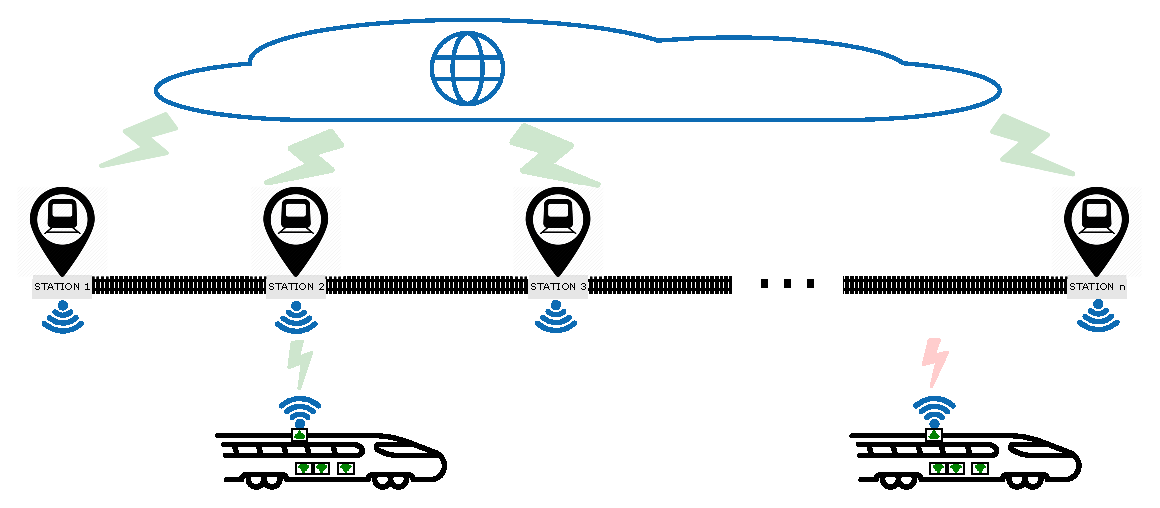
\includegraphics[width=1.0\textwidth,keepaspectratio]{figures/architecture}
	\caption{Architecture of proposed work.}
	\label{fig:41architecture}
\end{figure}







%%%%%%%%%%%%%%%%%%
%%%%%%%%%%%%%%%%%%
%%%%%%%%%%%%%%%%%%
%\newpage
\section{Non-intrusive self-powered sensor node}
\label{sec:42}
\subsection{Purpose}

The purpose of this section is to cover the acquisition and processing parts of the data-flow presented previously. As a starting point, a non-intrusive and self-powered sensor node allows the measurement of AC currents in all transformer secondary windings, as illustrated in figure \ref{fig:4.powerSensing}. This figure is based on the 3400 series train topology of \textit{Comboios de Portugal} (CP) used in urban services.

Based on the field measurements, a data concentrator will receive the current and voltage measurements from each sensor node. This data concentrator generates information based on the needed estimations and the acquisition of GPS location, as proposed by the European Commission regulation No 1301/2014. For each time-stamp, the active and reactive power is calculated and transmitted together with the geographical position.

In the scope of Shift2Rail, is expected to develop a smart metering system for RTS. Assuming that a non-intrusive measurement system is of extreme interest, this proposal of a non-intrusive and self powered sensor node goes along the goals of Shif2Rail.

On the field of measurement, non-intrusive technical solutions has been used for several years for current measurement, such as hall-effect current sensors, rogowsky probes or current transformers.
For self-powering purposes, some studies on using current transformers for energy harvesting has been proposed in the literature (\cite{ahola2008}, \cite{wu2013}, \cite{moon2015}, \cite{amaro2015}, \cite{brunelli2016}).


\begin{figure}[h!]
	\centering
	\vspace{-1em}
	\includegraphics[width=0.7\textwidth,keepaspectratio]{figures/4.Method/powerSensing}
	\caption{Power architecture of case-study train.}
	\label{fig:4.powerSensing}
\end{figure}






\subsection{Methodology}

The methodology is divided into two parts. The first part will be related to the processing of the data generated by the sensor nodes and the second part is the definition of the sensor itself.

As a starting point of the methodology, it is expected to work on the \textbf{development of models using simulation frameworks} similar to the ones presented in figure \ref{fig:4.methodElectrical}. The modeling of such architecture allows the evaluation of the power contribution of a train, at a certain instant, to the power injected to the catenary. This methodology will contribute to \textbf{simulation and implementation of processing algorithms} in the train data concentrator that, based on the measurement of AC secondary winding's voltages and currents, will generate the accurate value of the energy injected in the catenary by the traction substation. The expected result will be the comparison and validation of the energy injected into the catenary (retrieved from the traction substation meter) and the estimated energy (as the outcome of this part of work).
%The expected result will be the comparison between the estimation and the measured injected energy in the catenary.

In this second part of the methodology, or the acquisition part, the sensor will be defined and validated. As a first step in the methodology, using Ansys or similar Finit Element Method (FEM) software, the \textbf{current and electric field of one winding will be simulated}. With the results of this simulation, the current and voltage sensors will be evaluated. In a further step, \textbf{real experiments on low voltage test-bench} will test the proposed sensor node.



\begin{figure}[h!]
	\centering
	\includegraphics[width=0.9\textwidth,keepaspectratio]{figures/4.Method/methodElectrical}
	\caption{Models needed for simulation.}
	\label{fig:4.methodElectrical}
\end{figure}



\subsection{Simulation tools and frameworks}

\cite{pilo2000} identifies the need of two tools for the simulation of railway power lines: (1) the simulator for the railway line and (2) an electrical system simulator. Based on that, \cite{almagro2017} uses the simulation tool \textbf{OpenDSS} with the Python integration for the simulation of the railway power lines. A further study on OpenDSS shows enough documentation and recent updates (march 2017) with the possible integration with VBA Excel, MatLAB and Python scripts.

Mathworks suggests also the usage of \textbf{MatLAB and Simulink} for rail electrical systems modeling. 
Similarly, \textbf{Ansys} products are suggested for the simulation of railway power systems as well as \textbf{PSIM}. The three previously presented products are also flexible to work in co-simulation, with the advantage of choosing the best software for the most straightforward application.


	\subsection{Contributions}
	
	On the energy measurement and information generation of the sensor nodes, two contributions can be considered as follows:
	
	\begin{itemize}
		\setlength\itemsep{0em}
		
		\item \textbf{New energy metering architecture}, according to some specifications such as the usage of a non-intrusive approach.
		This architecture will generate energy information about the powerflow of the railway system.
		
		\item \textbf{Accurate estimation of power flow} into catenary, based on on-board measurements. The available parameters will be: (1) the RMS voltage, current and apparent power, (2) the instantaneous active power, reactive power, power factor and frequency, and (3) the cumulative energy consumptions in terms of kVAh, kVARh and KWh.
		
		
	\end{itemize}

%	\begin{itemize}
%		\setlength\itemsep{0em}
%		\item New energy metering architecture using a non-intrusive approach.
%		
%		\item Accurate estimation of injected power into catenary, that is needed for train operation, based on on-board measurements.
%		
%	\end{itemize}
	
%%%%%%%%%%%%%%%
%%%%%%%%%%%%%%%
%%%%%%%%%%%%%%%

\section{RTS wireless network}
\label{sec:43}

\subsection{Purpose}

The main purpose of the RTS wireless network is to transmit energy measurements and information generated by the nodes to a centralized storage server. 

As a lower level and as previously presented, each train has current sensors as nodes and a data concentrator. Between nodes and data concentrator, AC voltage and current measurements must be exchanged.
At this level, the relevant issue will be the presence of EMI, that will affect the communication link.

Between train data concentrator and ground-level, the train movement should be considered to better comply with the purpose of transmission the information generated at trains to the centralized storage server. 

Further modeling and simulation of a WSN for energy measurement of RTS rolling stock will be made.



\subsection{Methodology}

The methodology for this part will include the \textbf{modeling and simulation} of network blocks similar to the ones presented in figure \ref{fig:4.methodWireless}. An accurate modeling and simulation will define the more appropriate network technologies to implement in this RTS network. 
The simulation will be performed in a NS-3 simulator or similar.
The \textbf{results} of such simulation will define the max data-rate of the sensor nodes as well as the nodes energy consumption required for the information transmission.

\begin{figure}[h!]
	\centering
	\includegraphics[width=0.9\textwidth,keepaspectratio]{figures/4.Method/methodWireless}
	\caption{Models needed for simulation.}
	\label{fig:4.methodWireless}
\end{figure}

\subsection{Simulation tools and frameworks}

Several simulators/emulators were presented in the literature review chapter. From those, special attention is given to the NS-3 simulator and the MatLAB/Simulink tool.  
%<<necessário avaliar melhor os restantes candidatos>>


\subsection{Contribution}
%An energy measurement system in rolling stock does not require a broadband real-time/continuous communication (such as LTE), being possible to collect and store data in train data concentrator and, while the train is waiting at station for passenger exchange (which lasts for less than one minute), the data is transferred between train and station AP (and then to a remote server). Therefore, the contribution will be the cost reduction of information transmission of energy sensor network data

Regarding the energy information transmission and storage into centralized database, the following contributions are expected:

\begin{itemize}
	\setlength\itemsep{0em}
	
	\item \textbf{Availability of measured data} from trains where currently limited/inexistent energy measurement is performed.
	
	\item Data-rate increase of energy measurements, which will result on direct \textbf{increase on the quality of information of energy}. This increase will overcome the 5 minute data-rate that currently are used in energy meters.
	
\end{itemize}

A further contribution can be the reduction of the dependence of broadband real-time/continuous communication (such as LTE), with the direct cost reduction of information transmission of energy RTS data.

%\begin{itemize}
%	\setlength\itemsep{0em}
	
%	\item As a starting point, one contribution will be the availability of measured data from trains where currently no energy measurement is performed.
	
%	\item A second contribution will be the data-rate increasing of energy measurements, which will result on direct increase on the quality of information of energy.
	
%	\item A further contribution can be the avoidance of broadband real-time/continuous communication (such as LTE), being possible to collect and store data in train data concentrator and, while the train is waiting at stations, the data is transferred between train and station AP (and then to a remote server). A possible contribution will be the cost reduction of information transmission of energy sensor network data.
%\end{itemize}

\newpage
\section{Work plan}
\label{sec:44}

Based on the before-mentioned objectives, an annual planning for future developments was built for the next three years. 
The work plan is presented in Table \ref{workplan}. 


Secondary tasks of the work plan are the deliverables for the iRail programme and for the FCT institution, which occurs at end of academic year. 

% Please add the following required packages to your document preamble:
% \usepackage{booktabs}
% \usepackage{multirow}
\begin{table}[htbp]
	\centering
	\caption{Thesis work plan}
	\label{workplan}
	\footnotesize
	\setlength\extrarowheight{2pt}
	\resizebox{1.0\textwidth}{!}{ 
	\begin{tabular}{ccccc}
		\hline
%		\hline
		\textbf{Year}                            & \textbf{Semester}                         & \multicolumn{2}{c}{\textbf{Task}}                                                                                                                                                                                                                                                & \textbf{Milestone}                                                                                                  \\ \hline \hline
		\multicolumn{1}{|c|}{\multirow{6}{*}{1}} & \multicolumn{1}{c|}{\multirow{3}{*}{1st}} & \multicolumn{1}{c|}{\multirow{2}{*}{Train power model development}}                                                                      & \multicolumn{1}{c|}{\begin{tabular}[c]{@{}c@{}}Simulation of \\ traction power transformer\end{tabular}}                              & \multicolumn{1}{c|}{}                                                                                               \\ \cline{4-4}
		\multicolumn{1}{|c|}{}                   & \multicolumn{1}{c|}{}                     & \multicolumn{1}{c|}{}                                                                                                                    & \multicolumn{1}{c|}{\begin{tabular}[c]{@{}c@{}}Simulation of \\ train power system\end{tabular}}                                      & \multicolumn{1}{c|}{}                                                                                               \\ \cline{3-4}
		\multicolumn{1}{|c|}{}                   & \multicolumn{1}{c|}{}                     & \multicolumn{1}{c|}{\multirow{3}{*}{RTS energy model development}}                                                                       & \multicolumn{1}{c|}{Integration with real case-study}                                                                                 & \multicolumn{1}{c|}{}                                                                                               \\ \cline{2-2} \cline{4-4}
		\multicolumn{1}{|c|}{}                   & \multicolumn{1}{c|}{\multirow{3}{*}{2nd}} & \multicolumn{1}{c|}{}                                                                                                                    & \multicolumn{1}{c|}{\begin{tabular}[c]{@{}c@{}}Simulation of \\ railway power system\end{tabular}}                                    & \multicolumn{1}{c|}{}                                                                                               \\ \cline{4-4}
		\multicolumn{1}{|c|}{}                   & \multicolumn{1}{c|}{}                     & \multicolumn{1}{c|}{}                                                                                                                    & \multicolumn{1}{c|}{Algorithm implementation}                                                                                         & \multicolumn{1}{c|}{}                                                                                               \\ \cline{3-4}
		\multicolumn{1}{|c|}{}                   & \multicolumn{1}{c|}{}                     & \multicolumn{1}{c|}{\multirow{2}{*}{\begin{tabular}[c]{@{}c@{}}Energy measurement system:\\ node development\end{tabular}}}              & \multicolumn{1}{c|}{\begin{tabular}[c]{@{}c@{}}Hardware development of\\ Energy Measurement Node\end{tabular}}                        & \multicolumn{1}{c|}{}                                                                                               \\ \cline{1-2} \cline{4-5} 
		\multicolumn{1}{|c|}{\multirow{6}{*}{2}} & \multicolumn{1}{c|}{\multirow{3}{*}{1st}} & \multicolumn{1}{c|}{}                                                                                                                    & \multicolumn{1}{c|}{\begin{tabular}[c]{@{}c@{}}Results acquisition: \\ test bench validation of\\ Energy Measurement Node\end{tabular}} & \multicolumn{1}{c|}{\begin{tabular}[c]{@{}c@{}}Publication(s):\\ Energy Measurement Node\end{tabular}}                 \\ \cline{3-5} 
		\multicolumn{1}{|c|}{}                   & \multicolumn{1}{c|}{}                     & \multicolumn{1}{c|}{\multirow{3}{*}{\begin{tabular}[c]{@{}c@{}}RTS wireless smart \\ metering network\\ model development\end{tabular}}} & \multicolumn{1}{c|}{Model simulation}                                                                                                 & \multicolumn{1}{c|}{}                                                                                               \\ \cline{4-4}
		\multicolumn{1}{|c|}{}                   & \multicolumn{1}{c|}{}                     & \multicolumn{1}{c|}{}                                                                                                                    & \multicolumn{1}{c|}{Integration with real case-study}                                                                                 & \multicolumn{1}{c|}{}                                                                                               \\ \cline{2-2} \cline{4-5} 
		\multicolumn{1}{|c|}{}                   & \multicolumn{1}{c|}{\multirow{3}{*}{2nd}} & \multicolumn{1}{c|}{}                                                                                                                    & \multicolumn{1}{c|}{\begin{tabular}[c]{@{}c@{}}System integration with \\ energy measurement nodes\end{tabular}}                      & \multicolumn{1}{c|}{\begin{tabular}[c]{@{}c@{}}Publication(s): \\ RTS wireless \\ smart metering network\end{tabular}} \\ \cline{3-5} 
		\multicolumn{1}{|c|}{}                   & \multicolumn{1}{c|}{}                     & \multicolumn{1}{c|}{\multirow{3}{*}{System integration}}                                                                                 & \multicolumn{1}{c|}{\begin{tabular}[c]{@{}c@{}}Development of energy data\\ storage system;\end{tabular}}                             & \multicolumn{1}{c|}{}                                                                                               \\ \cline{4-4}
		\multicolumn{1}{|c|}{}                   & \multicolumn{1}{c|}{}                     & \multicolumn{1}{c|}{}                                                                                                                    & \multicolumn{1}{c|}{\begin{tabular}[c]{@{}c@{}}System integration:\\ RTS wireless smart metering network\end{tabular}}                & \multicolumn{1}{c|}{}                                                                                               \\ \cline{1-2} \cline{4-5} 
		\multicolumn{1}{|c|}{\multirow{6}{*}{3}} & \multicolumn{1}{c|}{\multirow{3}{*}{1st}} & \multicolumn{1}{c|}{}                                                                                                                    & \multicolumn{1}{c|}{\begin{tabular}[c]{@{}c@{}}Results acquisition: \\ Railway Smart Meter\end{tabular}}                               & \multicolumn{1}{c|}{\begin{tabular}[c]{@{}c@{}}Publication(s):\\ Railway Smart Meter\end{tabular}}                     \\ \cline{3-5} 
		\multicolumn{1}{|c|}{}                   & \multicolumn{1}{c|}{}                     & \multicolumn{1}{c|}{\multirow{5}{*}{Thesis Delivery}}                                                                                    & \multicolumn{1}{c|}{\multirow{4}{*}{Document writing}}                                                                                & \multicolumn{1}{c|}{}                                                                                               \\
		\multicolumn{1}{|c|}{}                   & \multicolumn{1}{c|}{}                     & \multicolumn{1}{c|}{}                                                                                                                    & \multicolumn{1}{c|}{}                                                                                                                 & \multicolumn{1}{c|}{}                                                                                               \\ \cline{2-2}
		\multicolumn{1}{|c|}{}                   & \multicolumn{1}{c|}{\multirow{3}{*}{2nd}} & \multicolumn{1}{c|}{}                                                                                                                    & \multicolumn{1}{c|}{}                                                                                                                 & \multicolumn{1}{c|}{}                                                                                               \\ \cline{5-5} 
		\multicolumn{1}{|c|}{}                   & \multicolumn{1}{c|}{}                     & \multicolumn{1}{c|}{}                                                                                                                    & \multicolumn{1}{c|}{}                                                                                                                 & \multicolumn{1}{c|}{Thesis Delivery}                                                                                \\ \cline{4-5} 
		\multicolumn{1}{|c|}{}                   & \multicolumn{1}{c|}{}                     & \multicolumn{1}{c|}{}                                                                                                                    & \multicolumn{1}{c|}{Public Presentation}                                                                                              & \multicolumn{1}{c|}{Public Presentation}                                                                            \\ \hline
	\end{tabular}
}
\end{table}






%\chapter{Preliminary Work}
%\input{chapters/4.Preliminary}



\bibliographystyle{chicago}
%chicago}

%nota: não ter espaços entre ficheiros
\bibliography{bib/outliers,bib/shift2rail,bib/references,bib/31.SmartM,bib/32.WirelessN,bib/33.EnergyS,bib/34.PowerS,bib/35.DSS,bib/36.OutlierD}
%\bibliography{outliers}
%\PrintBib{outliers, }


%\bibliographystyle{plainnat}
%\bibliography{references}

%\chapter*{Attachment 1 --- \large{Overview of communication systems for Smart Grids}}
%\includepdf[pages=-, scale=0.9, offset=-10 0, pagecommand={\thispagestyle{plain}}]  {chapters/communication}


\end{document}